\documentclass[UTF8]{ctexart}

\usepackage{subfiles}  

%下面的语句, 引入你的头部设置文件
\usepackage{C:/phpStorm_proj/02_myself_ID_EGO/+100_latex_all_math_sel/myPreamble} 
%必须是绝对路径,才能让各个tex在单独编译时使用到

\title{文件名}


%---------------------------------


\begin{document}
	\tableofcontents % 生成目录
	\date{} % 若不写这句, 则默认也会渲染出日期, 所以我们要手动赋空值
	\maketitle  %这行代码, 让你前面的 title, author, date生效
	
		
	

\section{ 随机变量 random variable}
	
	随机变量: 常用大写字母X,Y,Z 或希腊字母来表示. \\
	随机变量的取值 : 用小写字母 x,y,z等表示. \\
	
比如, 随机变量X,  其=a的话, 我们就把这个事件记作 $\{X=a\}$.  其概率就是 $ P\{X=a\}$, 或写作 $P(X=a)$. \\







	
\section{概率函数 : PMF (离散型数据的, 称为``概率质量函数 Probability mass function") \& PDF (连续性数据的, 称为``概率密度函数 Probability Density Function")}	




\subsection{离散型数据的 PMF}

描述``离散型数据"的概率分布情况 的曲线, 称为``概率质量函数"(PMF). \\

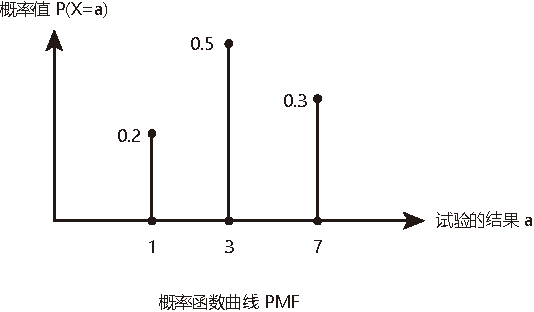
\includegraphics[width=0.6\textwidth]{/0116.pdf} \\

比如,掷骰子, 不同点朝上的概率为:$
\underset{\text{骰子在第}i\text{点的概率}}{\underbrace{p_i}}=\underset{\text{随机变量}X\text{在第}i\text{点时的概率}}{\underbrace{P(X=a_i)}},\ \ i\in 1,2,3,4,5,6
$ \\

在上面这个函数里 : \\
- 自变量X : 是``随机变量"的取值. \\
- 因变量  $ p_i$ 是``自变量X所取到某个值 $a_i$"的概率. \\

从公式上来看, \textbf{``概率函数", 一次只能表示一个取值的概率.} 比如 $ P(X=1)= 1/6$ 就表示: 当随机变量X 取值为 1时 (即骰子投到点数为1时) 的概率为1/6. 所以说, 它一次只能代表``随机变量的一个取值"的概率. \textbf{(即: P后面的小括号里, 只能写成 X= ..., 而不能写成 X>... 或 X<..., 大于小于符号这些, 就是属于``累加函数"了.)}\\



典型的``离散概率分布"包括: 伯努利分布,二项分布,几何分布,泊松分布等. \\





\subsection{连续性数据的 PDF}

``连续型数据"的概率分布, 称为``概率密度函数"(PDF).  \\


``概率密度函数"的 某区间上的概率值 = 该区间的函数曲线段, 与x坐标轴之间围成的面积. 实际上就是对``概率密度函数"进行定积分. \\


典型的``连续概率分布"包括: 正态分布, 指数分布等.



~\\
\hrule
~\\

\section{累积函数 $F(x)= P\{X \leq x\}$ : Cumulative Distribution Function (CDF)  ← 是对``概率函数"值的累加结果}

对于随机变量, 我们通常关心的, 并不是它取某个值的概率(即我们并不关心它的分布律), 而是更关心它落在某个区间内的概率.  \\
比如, 对某考试, 我们更关心的是``不及格的总人数", 和比如 ``分数≥80分 的总人数". \\

 在这些个区间段所占的概率值, 就是用``累加函数"(又叫``分布函数")来表示的. 即: \\
 $ (\text{随机变量}X\leq \text{自变量}x)=\underset{\text{累加函数}}{\underbrace{F(x)}}
$ ← 它表示随机变量X 落在 (-∞, x] 这段区间上的概率. \\
\vspace{1em} \\

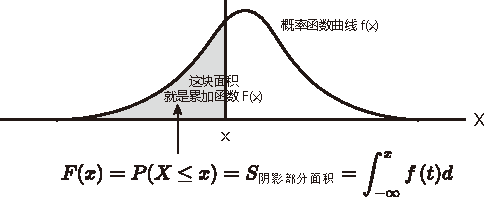
\includegraphics[width=0.7\textwidth]{/0125.pdf} \\



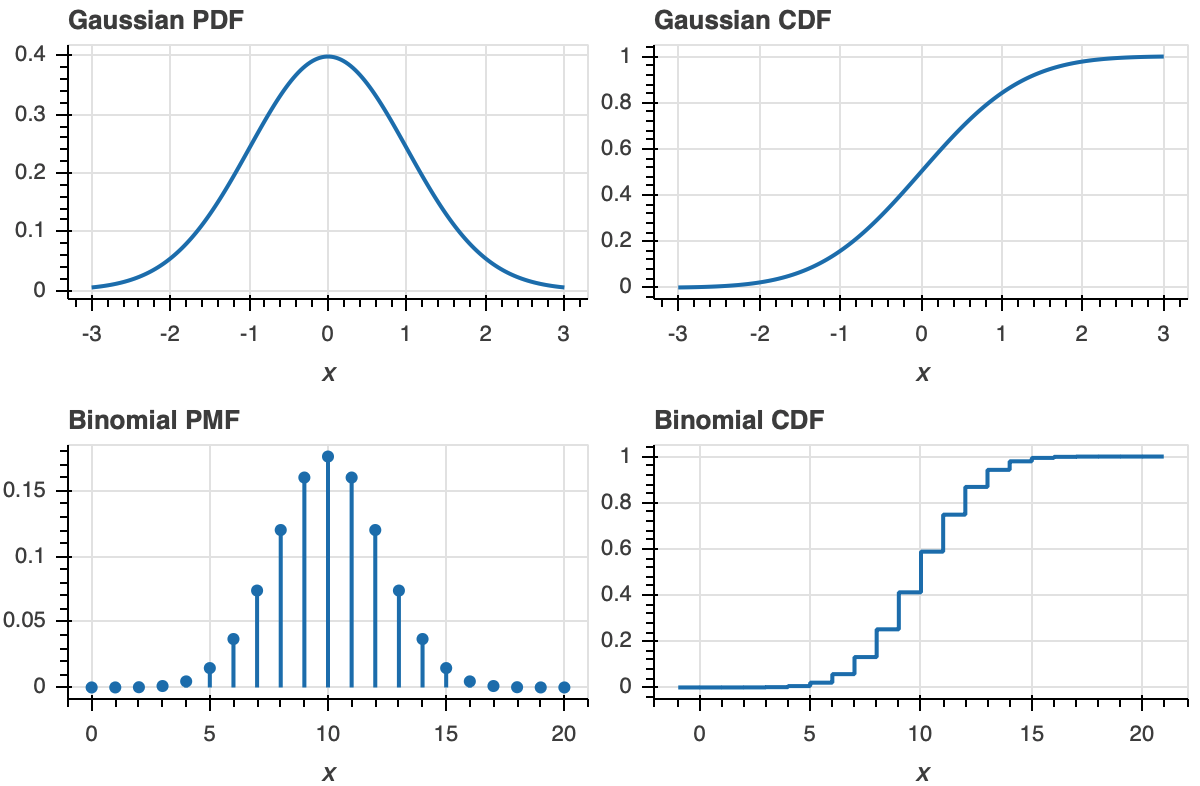
\includegraphics[width=1\textwidth]{/0117.png} \\

上图, 左边两张是``概率函数", 右边两张就是``累加函数 CDF". \\


累积函数 Cumulative Distribution Function (CDF) ← 是对``概率函数"值的累加结果 . 即对``概率密度函数"的积分.  \\

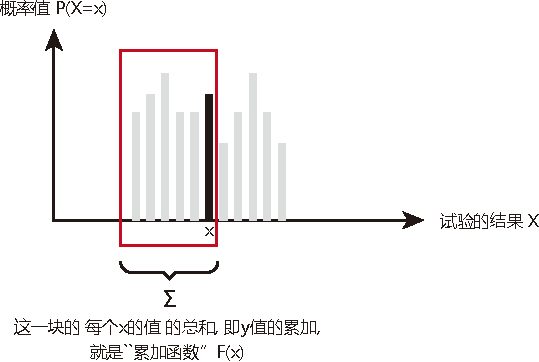
\includegraphics[width=0.7\textwidth]{/0118.pdf} \\


\begin{myEnvSample}
下面的图, 左边是``概率函数", 右边是``累加函数". \\

离散型数据的: \\
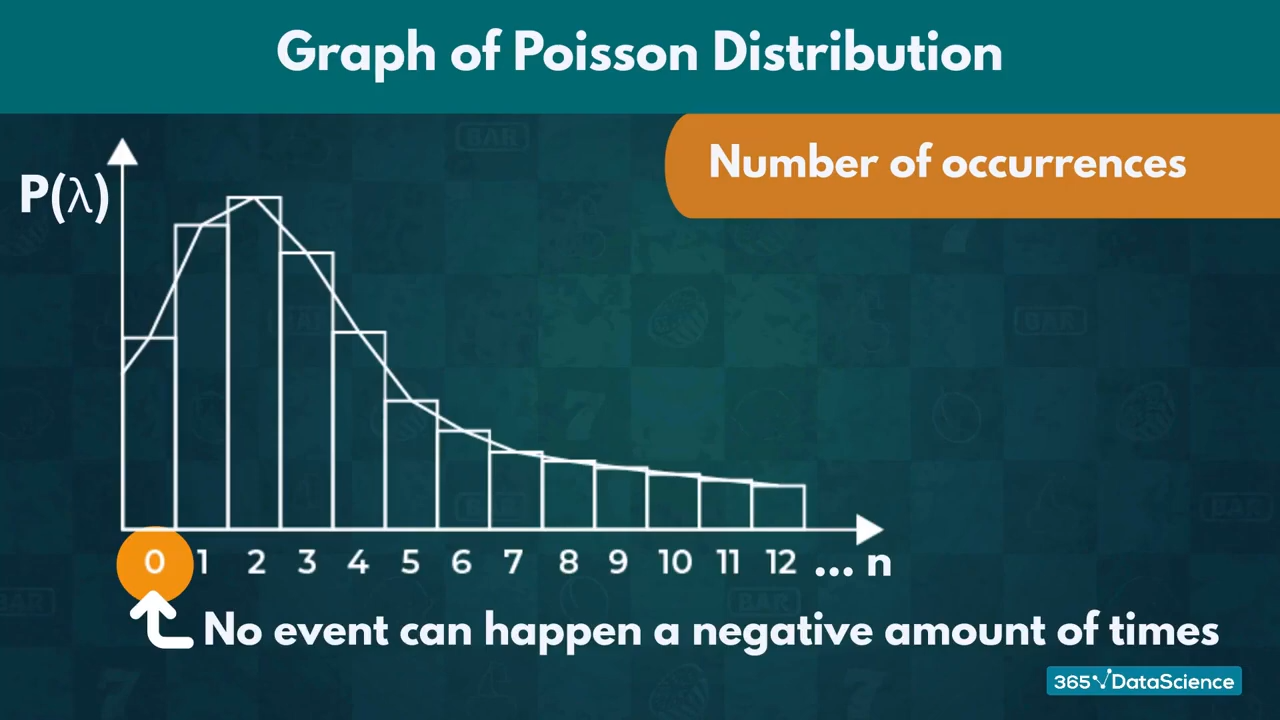
\includegraphics[width=0.8\textwidth]{/0122.png} \\

连续型数据的: \\
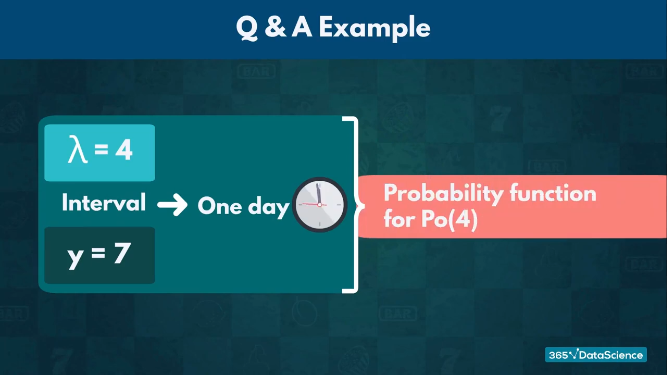
\includegraphics[width=0.8\textwidth]{/0123.png} \\


对``概率函数f(x)"求积分, 就得到``累加函数 F(x)" \\
对``累加函数 F(x)" 求导, 就得到``概率函数f(x)". \\

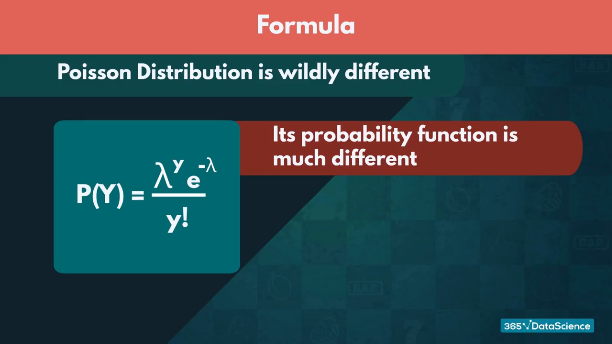
\includegraphics[width=0.8\textwidth]{/0124.png}
\end{myEnvSample}




	累加函数 : \\
	$ \boxed{
	F(x)=P(X\leq a)=\int_{lower\lim it}^a{f\left( x \right) dx}	}$ \\
	\\
	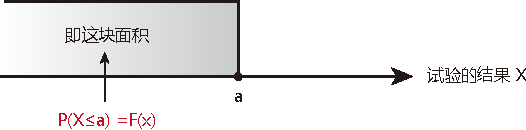
\includegraphics[width=0.6\textwidth]{/0119.pdf} \\
	
	
	$ \boxed{
	P(a\leq X\leq b)=P(a<X<b)=\int_a^b{f\left( x \right) dx}=F\left( b \right) -F\left( a \right) 	} $ \\
\\
	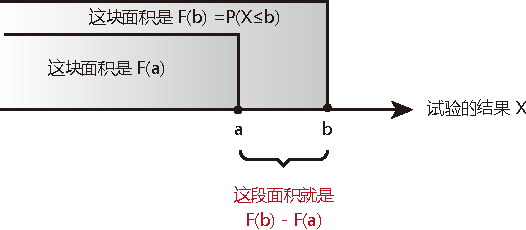
\includegraphics[width=0.6\textwidth]{/0120.pdf} 
	
	
	\begin{align*}  % 支持每行编号. 若不需要编号, 就用 align*环境
	& P(x_1<X\leq x_2)\ ←\ \text{对于随机变量}X\text{在}(x_1,x_2]\text{这段区间上的概率,它的值}\\
& =F(x_2)-F(x_1)\\
& =P\{X\leq x_2\}-P\{X\leq x_1\}
	\end{align*}





\subsection{单调不减性: 即 对于任意的 $x_1 < x_2$, 有: $F(x_1) \leq F(x_2)$}

比如, ``分数小于等于70分的人" 其概率一定是小于等于 ``分数小于80分的人". 即 $F(70) \leq F(80)$.



\subsection{F(-∞)=0 , F(+∞)=1}

$
\underset{=P(X\leq -\infty )}{\underbrace{F(-\infty )}}=\lim_{x\rightarrow -\infty}F(x)=0
$ ← 称之为 ``不可能事件". \\

$
\underset{=P(X\leq +\infty )}{\underbrace{F(+\infty )}}=\lim_{x\rightarrow +\infty}F(x)=1
$ ← 称之为 ``必然事件". \\

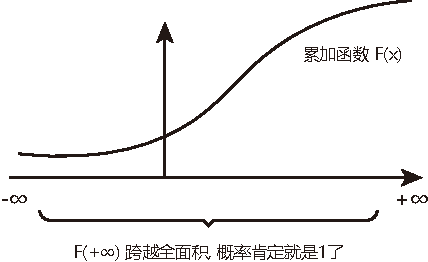
\includegraphics[width=0.5\textwidth]{/0121.pdf} \\


\subsection{右连续性: $\lim_{x -> x_0^+} F(x)=F(x_0)$ }


	
\end{document}